%%%
%%% CHAR(14)
%%%
%%% Lightning talk: pgloader
%%%

\documentclass{beamer}

\usepackage{minted}

\usepackage{beamerthemesplit}
\usepackage[utf8]{inputenc}
%% \usetheme{AnnArbor}
\usetheme{Boadilla}
%% \usetheme{Pittsburgh}
%% \usecolortheme{beaver}
%% \beamertemplatetransparentcovered

\title{pgloader}
\subtitle{PG DAY UK}
\author{Dimitri Fontaine \linebreak \url{@tapoueh}}
\date{July 9th, 2014}
\logo{
\includegraphics[height=0.4cm]{2ndQuadrant-cross.png}}

\begin{document}

\frame{\titlepage}

\begin{frame}
  \frametitle{Load data into PostgreSQL. Fast.}

  \center{\url{http://pgloader.io/}}

  \begin{center}
    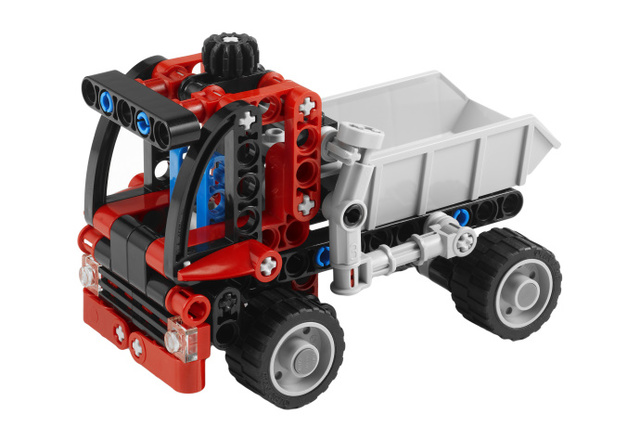
\includegraphics[height=2.1in]{pgloader.jpg}
  \end{center}
\end{frame}

\begin{frame}
  \frametitle{Load data into PostgreSQL. Fast.}

  \center{\url{http://pgloader.io/}}

  \begin{center}
    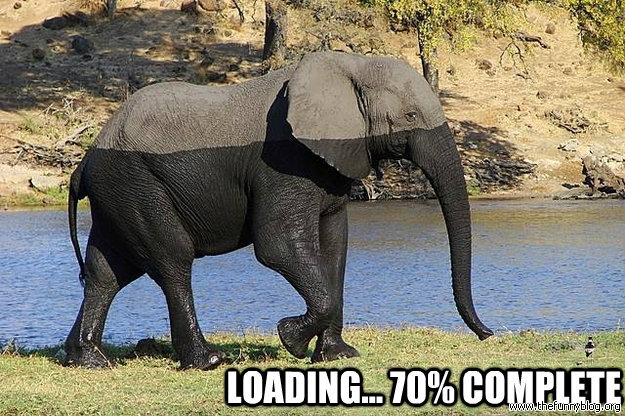
\includegraphics[height=2.1in]{elephant-loading.jpg}
  \end{center}
\end{frame}

\begin{frame}
  \frametitle{Load from CSV files}

  \center{\url{http://pgloader.io/howto/csv.html}}

  \begin{center}
    
\includegraphics[height=2.1in]{csv_text.png}
  \end{center}
\end{frame}

\begin{frame}
  \frametitle{Load from dBase III}

  \center{\url{http://pgloader.io/howto/dBase.html}}

  \begin{center}
    
\includegraphics[height=2.1in]{dBase.png}
  \end{center}
\end{frame}

\begin{frame}
  \frametitle{Load from SQLite}

  \center{\url{http://pgloader.io/howto/sqlite.html}}

  \begin{center}
    
\includegraphics[height=2.1in]{SQLite.png}
  \end{center}
\end{frame}

\begin{frame}
  \frametitle{Load from a live MySQL connection}

  \center{\url{http://pgloader.io/howto/mysql.html}}

  \begin{center}
    
\includegraphics[height=2.1in]{postgresql_versus_mysql.jpg}
  \end{center}
\end{frame}

\begin{frame}
  \frametitle{Load from a live MySQL connection}

  \center{\url{http://pgloader.io/howto/mysql.html}}

  \begin{center}
    
\includegraphics[height=2.1in]{mysql.png}
  \end{center}
\end{frame}

\begin{frame}
  \frametitle{pgloader : Transfom data on the fly}

  \center{\url{http://pgloader.io/}}

  \begin{center}
    
\includegraphics[height=2.1in]{huge-full-outer-join.jpg}
  \end{center}
\end{frame}

\begin{frame}
  \frametitle{Load data into PostgreSQL. Fast.}

  \center{\url{http://pgloader.io/}}

  \begin{center}
    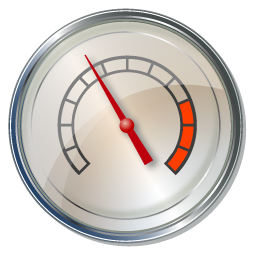
\includegraphics[height=2.1in]{performance-index-00.png}
  \end{center}
\end{frame}

\begin{frame}
  \frametitle{Used to be \textit{python} code. Now Common Lisp.}

  \begin{center}
    
\includegraphics[height=2.1in]{lisp-python.png}
  \end{center}
\end{frame}

\begin{frame}[fragile]
  \frametitle{pgloader got faster}

  \begin{minted}{postgresql}
 select rows, v2, v3,
        round((  extract(epoch from v2)
        / extract(epoch from v3))::numeric, 2)
        as speedup
   from timing;
        
  rows   |        v2         |       v3        | speedup 
---------+-------------------+-----------------+---------
 4768765 | @ 37 mins 10.878  | @ 1 min 26.917  |   25.67
 3115880 | @ 36 mins 5.881   | @ 1 min 10.994  |   30.51
 3865750 | @ 33 mins 40.233  | @ 1 min 15.33   |   26.82
 3994483 | @ 29 mins 30.028  | @ 1 min 18.484  |   22.55
(4 rows)
  \end{minted}
\end{frame}


\begin{frame}[fragile]
  \frametitle{Now using a command language}

  \begin{verbatim}
LOAD CSV
     FROM inline (x, y, a, b, c, d)
     INTO postgresql:///pgloader?csv (a, b, d, c)

     WITH truncate,
          skip header = 1,
          fields optionally enclosed by '"',
          fields escaped by double-quote,
          fields terminated by ','

      SET client_encoding to 'latin1',
          work_mem to '12MB',
          standard_conforming_strings to 'on'
  \end{verbatim}
\end{frame}

\begin{frame}[fragile]
  \frametitle{with extra before/after sections}

  \begin{verbatim}
   BEFORE LOAD DO
    $$ drop table if exists csv; $$,
    $$ create table csv (
        a bigint,
        b bigint,
        c char(2),
        d text
       );
    $$;
  \end{verbatim}
\end{frame}

\begin{frame}[fragile]
  \frametitle{Some data source examples}

  \begin{verbatim}
  FROM stdin
  FROM inline (a, b, c)
  FROM data/2013_Gaz_113CDs_national.txt
  
  FROM FILENAME MATCHING ~/GeoLiteCity-Location.csv/
  FROM ALL FILENAMES MATCHING ~/ALIOR/
  FROM ALL FILENAMES MATCHING ~/F[A-Z]{4}1[45]|OZ20/
  
  FROM http://www.census.gov/geo/maps-data/
              data/docs/gazetteer/places2k.zip
  
  FROM http://www.insee.fr/fr/methodes/nomenclatures/
                 cog/telechargement/2013/dbf/historiq2013.zip
\end{verbatim}
\end{frame}

\begin{frame}[fragile]
  \frametitle{Transformation de données}

  \begin{verbatim}
FROM FILENAME MATCHING ~/GeoLiteCity-Blocks.csv/
     WITH ENCODING iso-8859-1
     (
        startIpNum, endIpNum, locId
     )
INTO postgresql:///ip4r?geolite.blocks
     (
        iprange ip4r using (ip-range startIpNum endIpNum),
        locId
     )
  \end{verbatim}
\end{frame}

\begin{frame}
  \frametitle{MySQL et les types de données}

  \center{Text vide ou NULL, valeurs par défaut, dates à
    \texttt{0000-00-00}, \texttt{int(11)}, \texttt{float(20,2)},
    \texttt{tinyint} mais pas de \texttt{boolean}, \texttt{sets}, encodage,
    ... }
  
  \begin{center}
    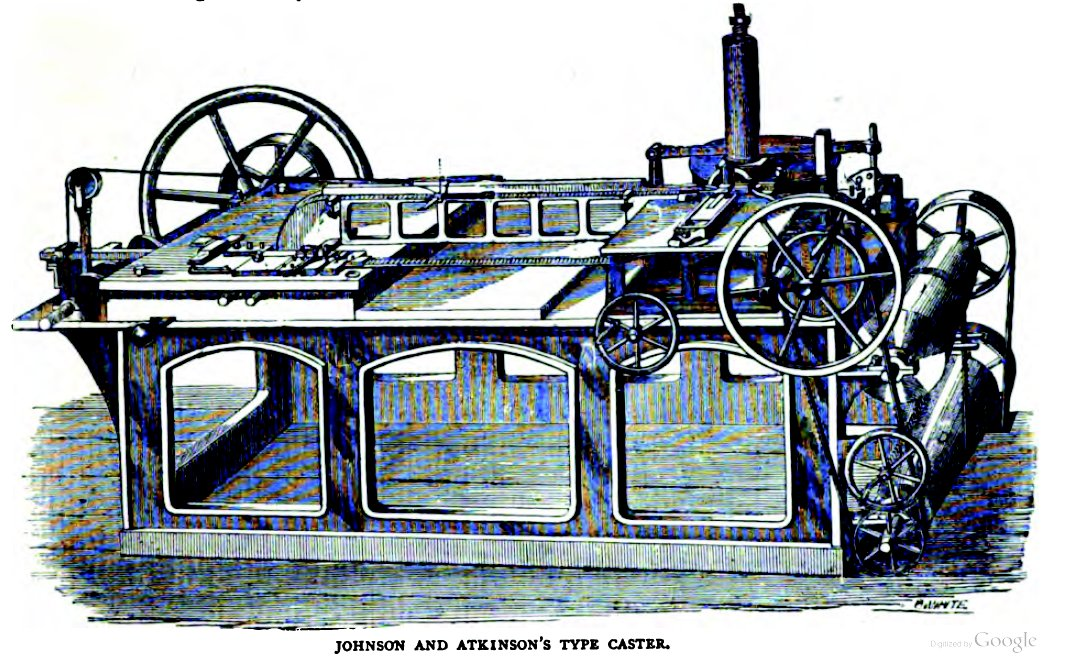
\includegraphics[height=2.1in]{type-casting-machine.jpg}
  \end{center}
\end{frame}

\begin{frame}
  \frametitle{Load data into PostgreSQL. Fast.}

  \center{\url{http://pgloader.io/}}

  \begin{center}
    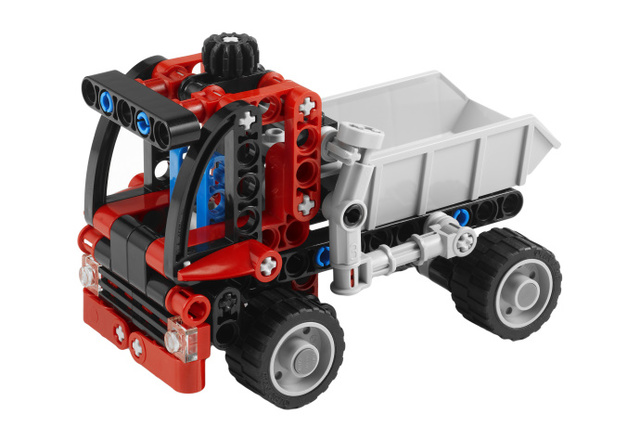
\includegraphics[height=2.1in]{pgloader.jpg}
  \end{center}
\end{frame}

\end{document}
